%!TEX root=../master.tex

\section{Partner attacking the Consumer}
The partner is an actor with relation to the consumer, but unlike the other actors partners usually can get away with more misdoings inside the consumer's property or house.

With this attack the partner wishes to monitor the consumer, possibly with following revenge, if monitoring leads to the conclusion that the consumer was cheating on the partner.
What distinguishes the partner's attacks from the burglar's and neighbour's is that the partner has increased access to the consumer's property, including the smart meter and related objects.

The attack trees are separated into the four modes of access for the same reasons as the burglar (see \cref{attacktree:burglar}) was.
The attack trees are listed below

These are listed below:
\begin{itemize}
  \item \Cref{fig:attack_trees:partner:cheater_sm}: Compromising the security on the smart meter.
  \item \Cref{fig:attack_trees:partner:cheater_client}: Compromising or extracting data from the device (the client) the consumer is using to communicate with the smart meter.
  \item \Cref{fig:attack_trees:partner:cheater_ecm}: Installing an ECM and monitoring the consumer.
  \item \Cref{fig:attack_trees:partner:cheater_physical}: Performing a \emph{``physical''} attack, involving no technology.
\end{itemize}

Each tree represents the possible attacks and gains, depending on the kind of access acquired.
There are two or three overall steps to the partner's attack plan: \textit{Gain access, Surveil, Get revenge}, which are repeated in the attack trees.

\begin{figure}[h]
  \centering
  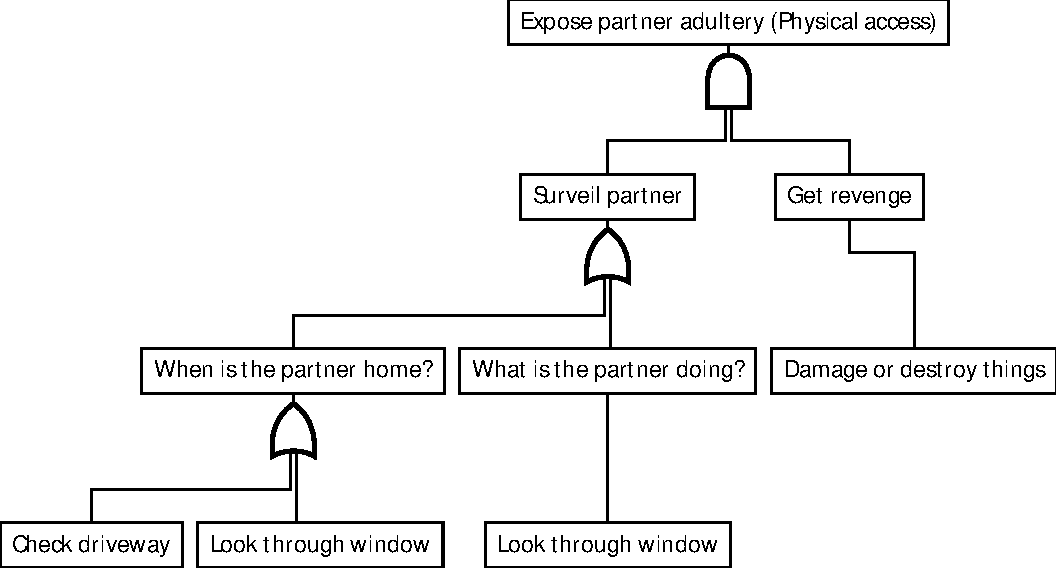
\includegraphics[width=\textwidth]{figures/graphviz/partner_vs_consumer_physical.pdf}
  \caption{The Partner attacking the Consumer by physical means.}
  \label{fig:attack_trees:partner:cheater_physical}
\end{figure}

\begin{figure}[h]
  \centering
  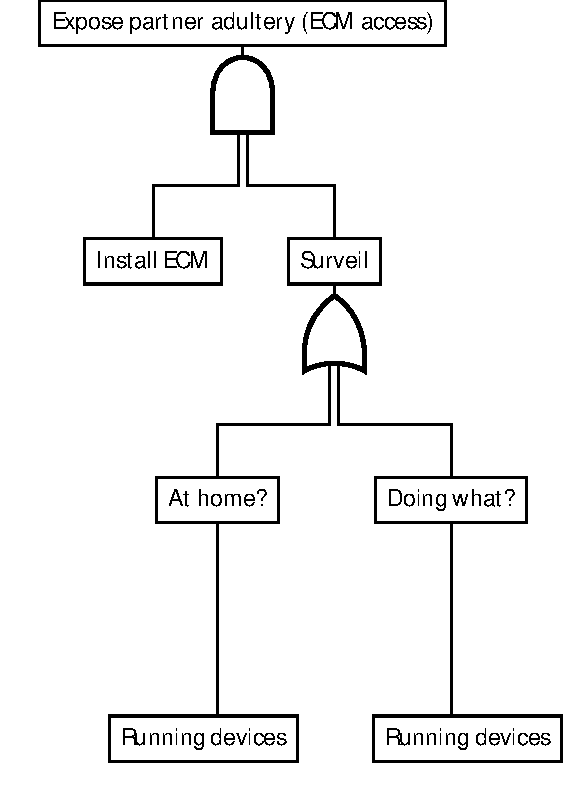
\includegraphics[width=\textwidth]{figures/graphviz/partner_vs_consumer_ecm.pdf}
  \caption{The Partner attacking the Consumer using an ECM.}
  \label{fig:attack_trees:partner:cheater_ecm}
\end{figure}

\afterpage{% Insert after the current page
\cleardoublepage
\thispagestyle{plain}
\KOMAoptions{paper=A3,paper=landscape}
\recalctypearea

\begin{figure}
  \centering
  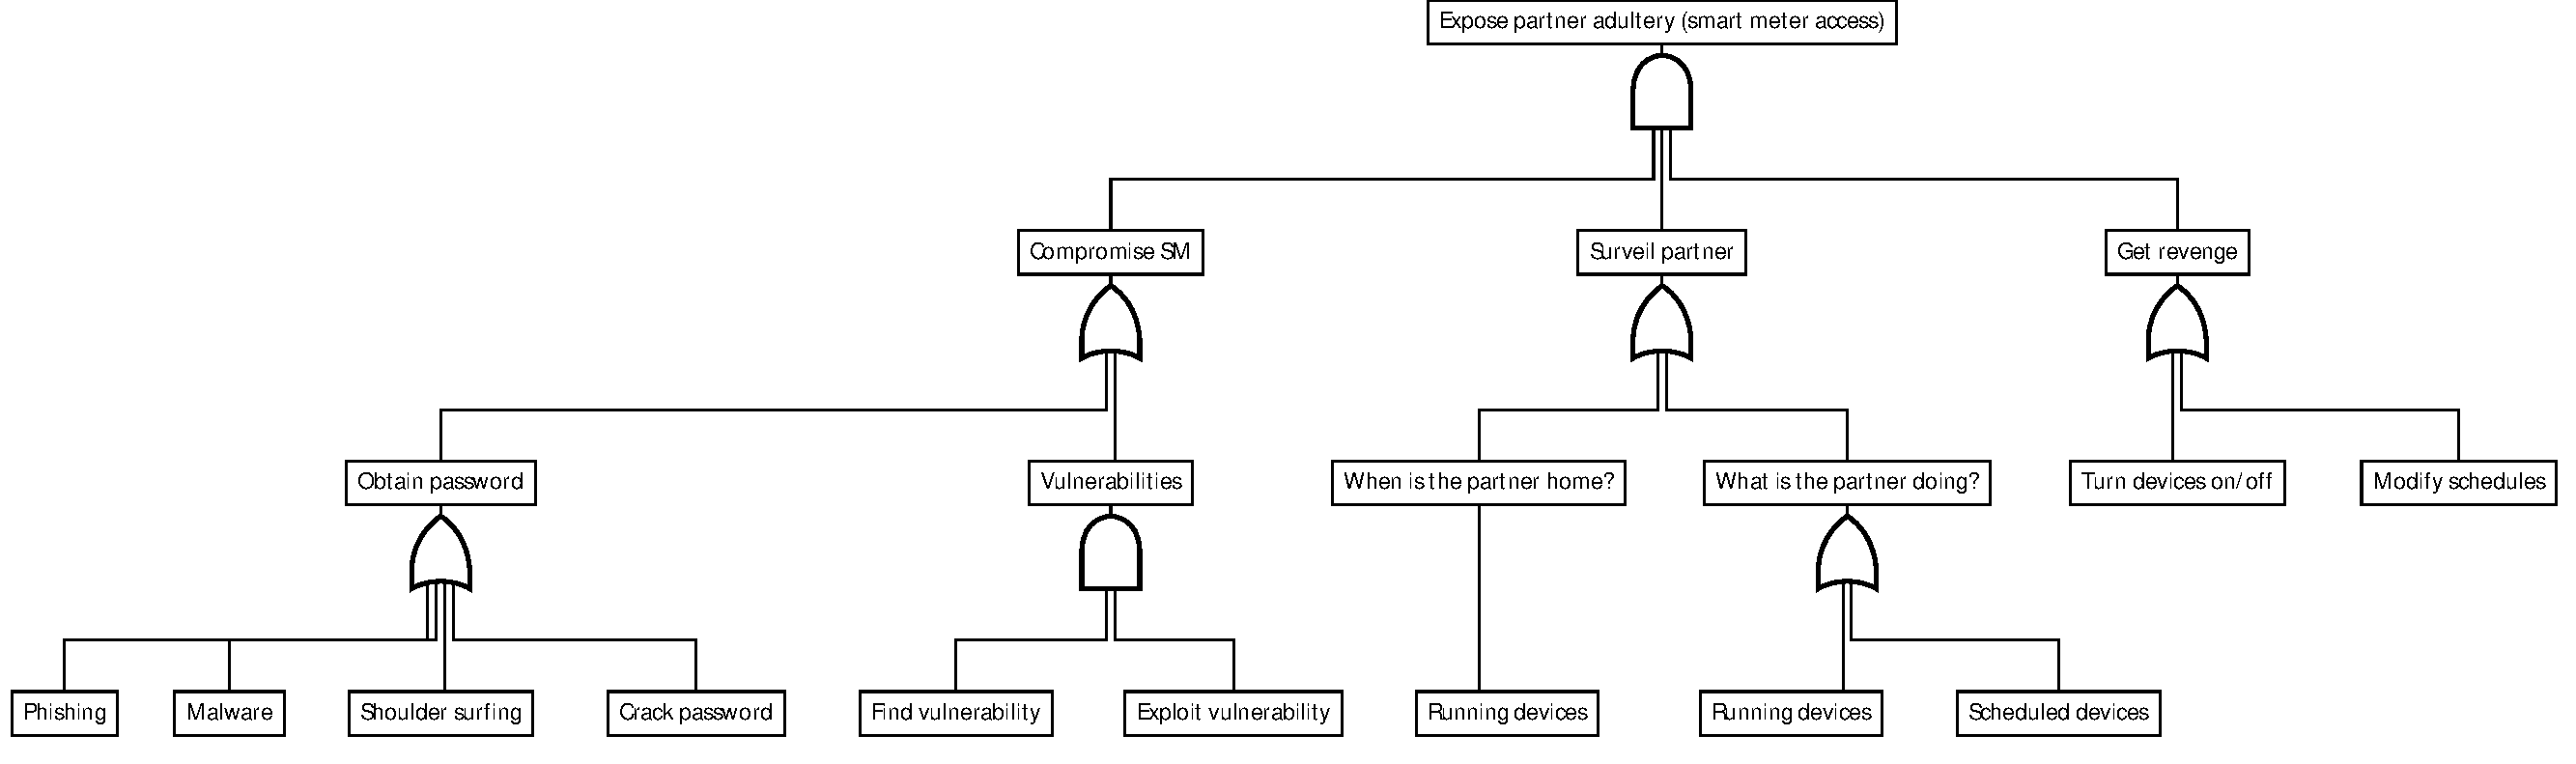
\includegraphics[width=\textwidth]{figures/graphviz/partner_vs_consumer_sm.pdf}
  \caption{The Partner attacking the Consumer by compromising his smart meter.}
  \label{fig:attack_trees:partner:cheater_sm}
\end{figure}

\cleardoublepage
\KOMAoptions{paper=A4,pagesize}
\recalctypearea
}

\begin{figure}
  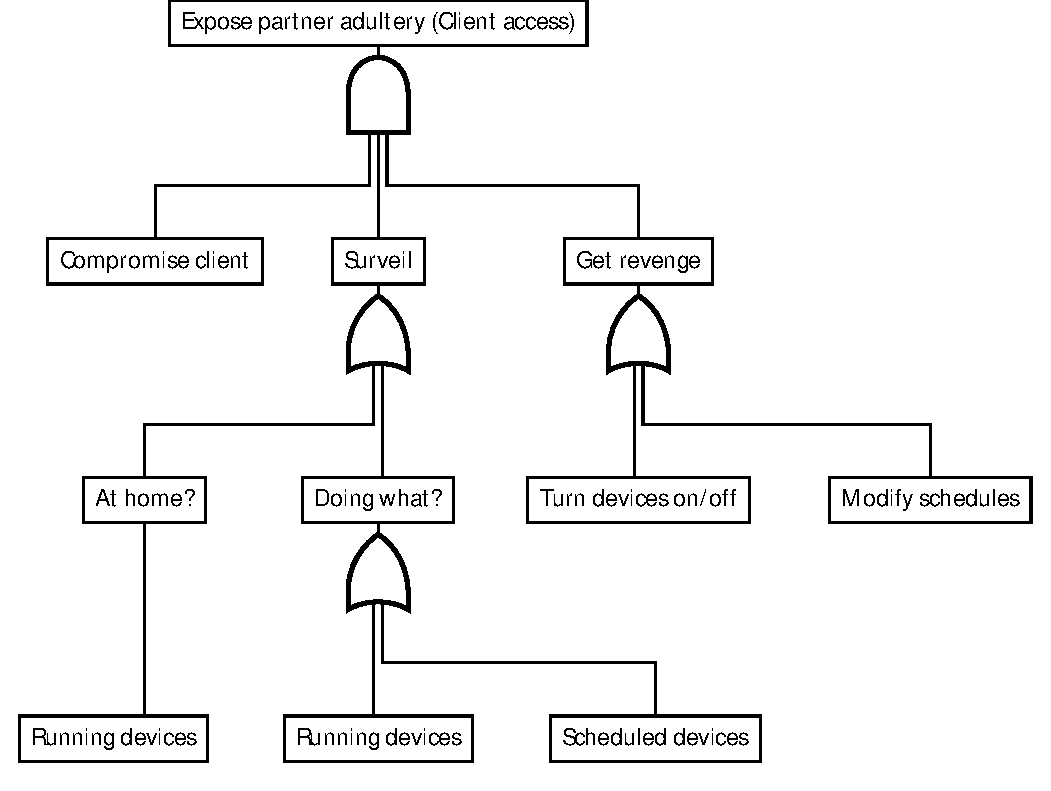
\includegraphics[width=\textwidth]{figures/graphviz/partner_vs_consumer_client.pdf}
  \caption{The Partner attacking the Consumer by compromising his client.}
  \label{fig:attack_trees:partner:cheater_client}
\end{figure}


\subsection{Access}
First of all the partner needs to gain access which can give the partner valuable insight into the doings of the consumer.
In relation to power consumption, the partner has three ways of accessing the consumer's data, which could give the partner the details the partner need to determine whether the consumer is home or not.

\subsubsection{Smart meter}
The first way is to compromise the smart meter.
This variation of the attack is identical to that of the burglar which was described in \cref{compromise:SM}.

\subsubsection{Client}
The other option is to gain access to the client that the consumer uses to control the smart meter.
This variation is similiar to the attack of the burglar described ion \cref{compromise:client}, with the exception that the partner has easier access to the client device.
A situation may arise where the partner has access to the client, and can then copy data from the device.

\subsubsection{ECM}
The partner could install an external consumption monitor\footnote{E.g. a TED (The Energy Detective) used in \cref {smart_meter_privacy}.} on the power grid in the house, giving the partner direct power consumption data.
This attack is similar to the burglar using an ECM described in \cref{compromise:ecm}.
Again the only variation is that the partner is closer to the consumer and therefore has more opportunities for installing the ECM.
For instance the partner could install it directly on the smart meter if the smart meter is hidden in a cupboard in the basement.

\subsection{Surveillance}
The main goal of this attack is to surveil and through this surveillance expose the consumer's misdeeds.
The nodes regarding devices are dependant on gained access through the \textit{Gain access} sub-tree as is represented with individual attack trees based on acquired access.

The partner's initial option is through a physical presence, such as looking through a window.
However, assuming that the partner was able to somehow get hold of the consumer's power consumption data, the partner now has options to expose the consumer from a distance.

First of all, the partner could determine whether the consumer is home, and shouldn't be, or that the consumer isn't home, but should be.
This can be done by looking at which devices are scheduled for tasks or from looking at the device power signatures.
The same method can be used to determine what the consumer is doing if the consumer is home, such as brewing more coffee than usual or taking unusually long showers.
See \cref{smart_meter_privacy} to see how to obtain this information from consumption data.

\subsection{Revenge}
The final step of the attack plan is an optional cold dish of revenge.

The partner could of course destroy stuff by applying physical manipulation in one way or another.
However, if the partner wanted to get creative, the partner could use the previously gained access to the smart meter to manipulate the consumer psychologically.
The partner could turn on/shut off the consumer's appliances at inconvenient times.
If the partner wanted to get even more creative, the partner could modify the appliances' schedules such as turning everything on at late night with low intervals.
